\documentclass[11pt]{article}
\usepackage[margin=1in]{geometry}
\usepackage{booktabs}
\usepackage{amsmath}
\usepackage{graphicx}
\usepackage{xcolor}
\usepackage{microtype}
\usepackage{listings}
\usepackage[hidelinks]{hyperref}
\lstset{basicstyle=\ttfamily\footnotesize,breaklines=true,columns=fullflexible,keepspaces=true}
\newcommand{\tps}{t/s}
\newcommand{\ds}{\textsc{ds4}}
\newcommand{\upstreamurl}{\url{https://github.com/antirez/ds4}}
% Fork with the branches and the reproduction package described in this paper.
\newcommand{\branchurl}{\url{https://github.com/parasol-aser/ds4}}

\title{Where the Tokens Go: Decomposing and Closing the Decode Gap for a 27B Hybrid LLM on Apple Silicon}
\author{Anonymous submission}
\date{Draft, September 2026}

\begin{document}
\maketitle

\begin{abstract}
On unified-memory Apple silicon, single-stream LLM decode is usually described
as memory-bandwidth bound, yet the most widely used runner reaches 45\% of the
nominal bandwidth roofline and 58\% of the measured streaming ceiling on
Qwen3.8-27B in Q4\_K. We decompose a decode token on an M2~Ultra into weight
streaming, matvec kernel efficiency, per-dispatch overhead, and CPU work on the
inter-token critical path, using command-buffer GPU timestamps rather than wall
clock so that sub-millisecond kernels are attributed correctly. Working inside
\ds{}, an open-source model-specific C/Metal engine, we add support for the
model and then apply three levers, each with a runtime switch so it can be
ablated: fewer bytes per token, fewer and better-shaped dispatches, and a
shorter CPU path between tokens. Decode rises from 29.3 to 33.1~\tps{}
(llama.cpp: 23.8), 81\% of the measured streaming ceiling, with logits that
match llama.cpp at an arbitrary decode step. A controlled comparison of Q4\_0
against Q4\_K on identical weights shows the block format is worth 7--19\% with
simple kernels and 1--2\% once the large matvecs are fused, because both
formats then stream at the same ceiling; MLX reaches the same rate on its
affine 4-bit format. We also fix a 2~ms-per-token sampler cost caused by
\texttt{isfinite} under \texttt{-ffast-math}, report three optimizations that
did not help and why, and release the code, switches and scripts.
\end{abstract}

\section{Introduction}

A 27B-parameter model in 4-bit quantization occupies about 15~GB, and a
single-stream decode step reads all of it. On an M2~Ultra (800~GB/s nominal)
the roofline is therefore about 53~\tps{}. llama.cpp decodes Qwen3.8-27B in
Q4\_K at 23.8~\tps{} on this machine (\S\ref{sec:eval}). More than half of the
token time is something other than moving weights, and the question this paper
answers is what.

The setting matters. Apple silicon is one of the few consumer platforms where
25--100B-parameter models fit in one address space, and people run such models
locally for chat, coding agents and private workloads. Its GPU is programmed
through Metal, kernels are dispatched from command buffers, and the CPU shares
the memory system, so CPU work between tokens delays the next submission. None
of the standard CUDA decode analyses transfer directly.

Our contributions are:
\begin{enumerate}
\item \textbf{A decomposition method for Metal decode} that attributes token
  time to weight streaming, matvec efficiency, per-dispatch overhead and CPU
  gaps (\S\ref{sec:method}). Stage timing uses the GPU start and end
  timestamps of command buffers; timing on the CPU carries a ${\sim}0.16$~ms
  synchronization floor that is larger than most of the kernels being
  measured.
\item \textbf{Optimizations, each measured in isolation}, organized by lever
  (\S\ref{sec:opt}, Table~\ref{tab:ablation}): a multi-weight matvec that
  issues a layer's side projections as one launch, a vectorized Q4\_K inner
  loop, residual add fused into the following RMSNorm, a single-launch
  attention prologue, a context-scaled split-KV attention, and a sampler
  rewrite. Switching all of them off reproduces the pre-optimization baseline
  exactly.
\item \textbf{A controlled quantization-format experiment}
  (\S\ref{sec:q40}) using the same weights in Q4\_0 and Q4\_K, in two engines
  and at two kernel-fusion levels.
\item \textbf{Negative results with mechanisms} (\S\ref{sec:negative}) and a
  correctness protocol that compares logits with the reference implementation
  at an arbitrary decode step (\S\ref{sec:correctness}).
\end{enumerate}

The engine is \ds{} (DwarfStar), an open-source model-specific inference engine
in C and Metal by Salvatore Sanfilippo and contributors~\cite{ds4}
(\upstreamurl{}). It
implements a handful of architectures as hand-written graphs rather than
interpreting a generic GGUF computation graph. Our work adds Qwen3.8-27B to it,
including the Gated DeltaNet and gated-attention kernels, and the decode paths
and measurements described below; the code, the runtime switches and the
experiment scripts are at \branchurl{}. We argue in \S\ref{sec:discussion}
that the model-specific trade is the right one for the small set of models
that people actually run locally.

\section{Background}
\label{sec:background}

\subsection{Platform}
The M-series SoCs share one LPDDR5 pool between CPU and GPU. Metal compiles
kernels at runtime from Metal Shading Language and executes them from command
buffers; a compute encoder can hold many dispatches, which execute serially with
memory ordering. There is no host-to-device copy, but the CPU and the GPU share
bandwidth, and the CPU-side work between two tokens is on the critical path.

All measurements are on a Mac Studio with an M2~Ultra (24 CPU cores, 60 GPU
cores, 192~GB LPDDR5, 800~GB/s nominal) running macOS 26.1 with Apple clang 17.
Baselines are llama.cpp at commit \texttt{6d9c82ea2} (2026-09-09) with its
Metal backend~\cite{llamacpp}, and mlx-lm 0.31.3~\cite{mlxlm}. All GGUF
engines read the same files from the Unsloth release~\cite{unslothdynamic};
MLX uses the community 4-bit conversion of the same checkpoint.

\subsection{Model}
Qwen3.8-27B (GGUF architecture \texttt{qwen35}) is a dense hybrid of 64
layers~\cite{qwen35}. In three layers out of four the token mixer is Gated
DeltaNet~\cite{yang2025gateddeltanet}: one fused projection produces $q$, $k$
(16 heads of 128) and $v$ (48 heads of 128) that share a causal depthwise
convolution of width 4; each value head keeps a $128\times128$ recurrent state
updated by the delta rule with a scalar per-head decay $\exp(A\cdot
\mathrm{softplus}(\alpha+b))$ and a write strength $\sigma(\beta)$, where
$\alpha$ and $\beta$ come from two 48-wide projections; the output is
RMS-normalized per head and gated by $\mathrm{SiLU}(z)$ from a 6144-wide
projection. Every fourth layer is gated grouped-query attention: 16 query
heads of dimension 256 with 4 KV heads, NEOX RoPE on the first 64 dimensions,
per-head RMSNorm on $q$ and $k$, and the output multiplied by a sigmoid gate
that is projected alongside $q$. All layers have a SwiGLU FFN of hidden size
17408; the width is 5120 and the vocabulary has 248,320 entries.
Table~\ref{tab:bytes} gives the bytes a decode step reads.

\begin{table}[t]
\centering
\begin{tabular}{lrr}
\toprule
Component & Weights & Q4\_K bytes \\
\midrule
DeltaNet layer ($\times$48): $qkv$, $z$, $\alpha$, $\beta$, out, FFN & 383.3M & 215.6~MB \\
Attention layer ($\times$16): $q|$gate, $k$, $v$, out, FFN & 372.3M & 209.4~MB \\
Layers total & & 13.70~GB \\
Output head, Q8\_0 ($248320\times5120$) & 1.27B & 1.35~GB \\
\midrule
Per token & & 15.05~GB \\
\bottomrule
\end{tabular}
\caption{Bytes streamed per decode token for Qwen3.8-27B in pure Q4\_K
(0.5625~B/weight) with a Q8\_0 output head (1.0625~B/weight). The token
embedding is read for one row only.}
\label{tab:bytes}
\end{table}

\subsection{Roofline}
At 15.05~GB per token the nominal bound is 53~\tps{}. The practical ceiling is
what the GPU actually streams: the fastest kernel we observe is the Q8\_0
output-head matvec at 670~GB/s (1.35~GB in 2.01~ms), and the fastest Q4\_K
kernel reaches 613~GB/s. Taking 620~GB/s as achievable gives 24.3~ms per token,
or 41~\tps{}. We use 41~\tps{} as the ceiling throughout.

\section{Measurement method}
\label{sec:method}

\paragraph{Per-stage GPU spans.}
\ds{} can close and reopen its command buffer at named stage boundaries inside
a layer (projections, convolution and recurrence, attention, output
projection, FFN gate/up, FFN down, residual and norm) under an environment
switch. We time each stage with the command buffer's \texttt{GPUStartTime} and
\texttt{GPUEndTime}. Timing the same boundaries with the CPU clock, as the
engine's earlier profiler did, includes a synchronization of about 0.16~ms per
boundary, which is larger than the recurrence, the attention or any norm.
Isolating a stage in its own command buffer still adds a fixed per-buffer cost
of a few microseconds, so the sum over stages exceeds the unperturbed token
time by a few percent (30.9~ms against 30.2~ms for the final build); we use the
profile for ranking and for deltas, and unperturbed runs for throughput.

\paragraph{System traces.}
Metal System Trace (\texttt{xctrace}) records GPU busy intervals and
command-buffer submissions process-wide; from it we take GPU busy fraction,
GPU time per token and CPU encode time per token, for \ds{} and llama.cpp on
the same prompt.

\paragraph{CPU inter-token split.}
The CLI generation loop reports, under a switch, the wall time per token spent
in sampling, in token emission and in the forward call. Neither GPU view
exposes this, and it is where the sampler cost of \S\ref{sec:cpu} was found.

\paragraph{Reference logits.}
A small program on the llama.cpp API prefills a prompt, greedy-decodes, and
writes the full logit vector at a chosen step $k$; \ds{} writes the logits of
its $k$-th forward under a switch. We report mean and maximum absolute
difference over the 248,320 entries and whether the argmax agrees. With greedy
decoding on both sides the token histories are identical up to $k$ whenever the
argmax agreed at every earlier step, so the comparison exercises the decode
kernels, not only prefill.

\section{Anatomy of a decode token}
\label{sec:anatomy}

Table~\ref{tab:stages} is the per-stage profile of one decode token on the
final build with every optimization switched off and on, and Figure~\ref{fig:breakdown}
groups it. Three observations organize the rest of the paper.

\begin{table}[t]
\centering
\footnotesize
\begin{tabular}{llrrrrr}
\toprule
Layer & Stage & \multicolumn{2}{c}{Optimizations off} & \multicolumn{2}{c}{On} & On, 8.6k ctx \\
 & & $\mu$s/layer & ms/token & $\mu$s/layer & ms/token & ms/token \\
\midrule
both & FFN gate/up & 196.0 & 12.54 & 163.6 & 10.47 & 10.49 \\
both & FFN down & 111.5 & 7.14 & 94.6 & 6.05 & 6.05 \\
DeltaNet & projections $qkv$, $z$, $\alpha$, $\beta$ & 116.0 & 5.57 & 93.6 & 4.49 & 4.50 \\
attention & projections $q|$gate, $k$, $v$ & 95.5 & 1.53 & 81.5 & 1.30 & 1.30 \\
DeltaNet & output norm + out projection & 45.5 & 2.19 & 47.2 & 2.27 & 2.28 \\
attention & gate + out projection & 42.7 & 0.68 & 44.1 & 0.71 & 0.71 \\
DeltaNet & conv + recurrence & 23.7 & 1.14 & 23.6 & 1.13 & 1.13 \\
attention & split-KV attention (+pad, reduce) & 105.9 & 1.69 & 60.5 & 0.97 & 3.38 \\
attention & $q$/$k$ prologue, $V$ store & 7.6 & 0.12 & 7.4 & 0.12 & 0.13 \\
both & residual adds and norms & 28.3 & 1.82 & 21.7 & 1.39 & 1.40 \\
 & output head (Q8\_0) & & 2.01 & & 2.01 & 2.01 \\
\midrule
 & total & & 36.43 & & 30.92 & 33.39 \\
\bottomrule
\end{tabular}
\caption{GPU time per decode token by stage, Qwen3.8-27B pure Q4\_K, M2~Ultra,
40-token context, from the per-stage profiler on the final build. ``Off''
disables the six switches of Table~\ref{tab:ablation}; the unswitchable
single-launch prologue is present in both columns. The last column is the
``on'' build at an 8,590-token context. Each stage runs in its own command
buffer, so totals exceed the unperturbed token times (34.2 and 30.2~ms).}
\label{tab:stages}
\end{table}

\begin{figure}[t]
\centering
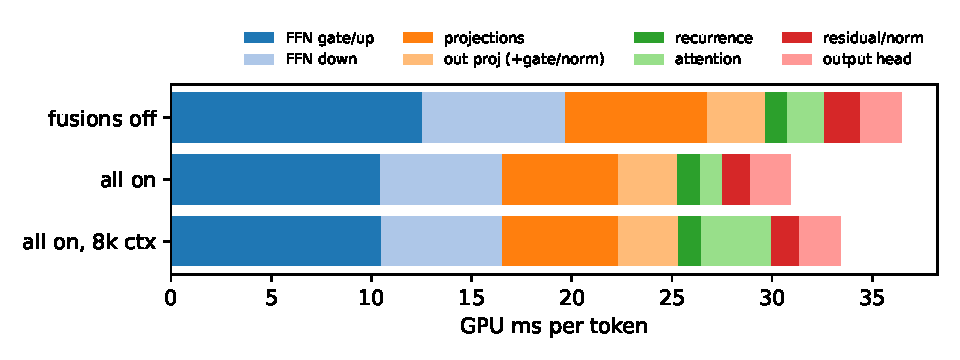
\includegraphics[width=0.9\linewidth]{figs/breakdown.pdf}
\caption{Table~\ref{tab:stages} grouped by stage type.}
\label{fig:breakdown}
\end{figure}

\paragraph{The large matvecs are near, not at, the ceiling.}
The FFN gate/up pair moves 100.3~MB per layer. As two ggml-style matvecs plus
a SwiGLU kernel it streams at 512~GB/s; fused and vectorized (\S\ref{sec:opt})
at 613~GB/s. The 5120-output projections (FFN down, attention and DeltaNet
output) sit at 390--450~GB/s with the ggml-style kernel. The Q8\_0 output head
reaches 670~GB/s on the same memory system, so part of the Q4\_K deficit is the
ALU cost of unpacking its 6-bit sub-block scales and minimums.

\paragraph{Dispatch count matters at this scale.}
The pre-optimization graph issued about 1,070 dispatches per token (16 per
DeltaNet layer, 19 per attention layer, plus embedding and head); at a few
microseconds of ramp and drain each this is 3--5~ms, as much as the
recurrence, the attention and all norms together. The final graph issues about
620.

\paragraph{GPU busy is not GPU useful.}
On the mixed-recipe UD-Q4\_K\_M file, the system trace shows \ds{} at 98.3\%
GPU busy against 95.6\% for llama.cpp, with about 1~ms of CPU encode time per
token against 4.9~ms. Both engines keep the GPU occupied; most of the gap to
the ceiling is inside kernels rather than between them, which is why the work
below is mostly about kernel shape and fusion.

\section{Optimizations by lever}
\label{sec:opt}

Every optimization below has an environment switch, so the final build can
reproduce any subset. Table~\ref{tab:ablation} and Figure~\ref{fig:ablation}
give the single-switch ablation; all switches off reproduces the original
29.2~\tps{}.

\subsection{Bytes: how fast a byte moves}
The format fixes the byte count; the kernel decides how close to the streaming
rate the bytes move. Two changes to the Q4\_K inner loop were worth 9.6\% on
the fused gate/up kernel (178.6 to 162.9~$\mu$s per layer): staging the 32
activation values a lane needs as eight \texttt{float4} loads instead of 32
scalar loads (the activation pointer's alignment is not provable to the
compiler, so it does not vectorize the loads itself), and loading each lane's
two 8-byte nibble runs as \texttt{uint2} instead of four \texttt{uint16}.
Amortizing one activation staging over four rows per simdgroup instead of two
helped the 10240- and 12288-output projections in the stage profile and hurt
the 5120-output ones, so the row count is chosen per shape; end to end the
difference is within noise (Table~\ref{tab:ablation}). A K-split variant,
which spreads one row's reduction over the simdgroups of a threadgroup and
combines through threadgroup memory, helps only the long-row FFN down
projection (17408 inputs: 111 to 94~$\mu$s) and is used only there.

\subsection{Dispatches: fewer and better shaped}
\paragraph{Multi-weight matvec.} A DeltaNet layer's four side projections
($qkv$, $z$, $\alpha$, $\beta$) share one activation and one input width. One
kernel with up to four weight segments, dispatched as a single grid whose
threadgroup ranges map to segments, writes the outputs back to back into the
existing batch buffer; the convolution and recurrence read $z$, $\alpha$ and
$\beta$ through views. The same kernel issues $q|$gate, $k$ and $v$ of an
attention layer. Four launches become one, and the 48-output $\alpha$ and
$\beta$ heads no longer each pay a dispatch.
\paragraph{Fused gate/up SwiGLU.} One kernel streams the gate and up weights
against one staged activation and writes $\mathrm{SiLU}(g)\cdot u$; the
elementwise SwiGLU pass disappears and the activation is read once per four
rows instead of once per two.
\paragraph{Residual add fused into the next norm.} Each residual add is fused
with the RMSNorm that consumes its result, so a layer's FFN epilogue produces
the next layer's attention-norm input and the two adds and two norms per
layer become two kernels.
\paragraph{Single attention prologue.} Per-head RMSNorm plus RoPE for the
query heads (to the f32 scratch), the same for the key heads (into the f16 K
cache) and the $V$ store are one grid with three kinds of threadgroup instead
of three launches.
\paragraph{Context-scaled split-KV.} The split-KV decode attention kernel
inherited from ggml partitions the keys over 32 workgroups and reduces their
partial results in a second kernel. At a 40-token context 30 workgroups are
idle and the reduce dominates. Scaling the workgroup count with the context
length, and letting a single workgroup write its normalized output directly,
cuts the attention stage from 106 to 61~$\mu$s per layer. This required making
the shared reduce kernel correct for fewer than 32 workgroups, which it had
silently assumed.

\subsection{The CPU path between tokens}
\label{sec:cpu}
With sampling at the model card's defaults (temperature 1.0, top-$p$ 0.95, no
top-$k$), the CLI spent 2.2~ms per token in the sampler against 30.4~ms in the
forward call. The cost was not the softmax or the sort but
\texttt{isfinite()} on each of the 248,320 logits: the engine is compiled with
\texttt{-ffast-math}, which on this toolchain leaves \texttt{isfinite} as a
library call and keeps the scan scalar at about 4~ns per element, twice per
token. A first replacement, an exponent-bit test on the float value, was folded
to ``always finite'' by the optimizer under the same flags, admitted NaN and
$-\infty$ logits, and failed 1,459 unit tests. The working version tests the
bits as loaded from memory, which the optimizer cannot classify. With the max
scan and the top-$p$ pass then written branch-free and block-wise so they
vectorize, a degree-5 fit of $2^x$ for the tail mass that cannot enter the
512-entry candidate heap, and a lowering-cutoff fallback instead of a
full-vocabulary sort, sampling costs 0.5~ms per token. The two lessons are
general: profile the inter-token gap on the CPU, and treat fast-math flags as
part of the numerical contract of any code that handles non-finite values.

\section{Correctness}
\label{sec:correctness}
Every change was checked against llama.cpp logits at decode step 4 on two
prompts (Table~\ref{tab:logits}); the values are identical across all
optimizations, and prefill logits are bit-identical between the initial and
final builds because no prefill kernel changed.

\begin{table}[t]
\centering
\begin{tabular}{lrrr}
\toprule
Prompt & mean $|\Delta|$ & max $|\Delta|$ & argmax \\
\midrule
22-token chat prompt & 0.012 & 0.179 & agrees \\
1439-token prompt & 0.024 & 0.214 & agrees \\
\bottomrule
\end{tabular}
\caption{Logit difference from llama.cpp at decode step 4, pure Q4\_K, over
248,320 entries.}
\label{tab:logits}
\end{table}

Because both engines read the same file and agree to this precision, the
quality of a file is a property of the quantization, not the engine.
Table~\ref{tab:ppl} gives wikitext-2 perplexity~\cite{merity2016pointer} per
file. The three GGUF recipes are indistinguishable within their standard
errors, so the 41\% decode advantage of pure Q4\_K over Q8\_0 in
Table~\ref{tab:tps} is free on this metric; the two affine 4-bit variants
(MLX, Q4\_0) cost 3--4\%.

\begin{table}[t]
\centering
\begin{tabular}{lrr}
\toprule
File & bytes/weight & wikitext-2 PPL \\
\midrule
pure Q4\_K, imatrix & 0.5625 & $5.80 \pm 0.07$ \\
UD-Q4\_K\_M & 0.58 & $5.85 \pm 0.07$ \\
Q8\_0 & 1.0625 & $5.86 \pm 0.07$ \\
MLX 4-bit affine, group 64 & 0.5625 & $5.98$ \\
pure Q4\_0, imatrix & 0.5625 & $6.03 \pm 0.07$ \\
\bottomrule
\end{tabular}
\caption{Perplexity on the first 40 chunks of 2048 tokens of wikitext-2 test,
scoring the second half of each chunk (\texttt{llama-perplexity} for the GGUF
files; a script with the same chunking for the MLX model, which reports no
standard error). Bytes per weight are for the layer tensors. The MLX
conversion uses no importance matrix.}
\label{tab:ppl}
\end{table}

\subsection{Downstream check}
\label{sec:downstream}
As a coarse check on reasoning tasks we ran \ds{}'s built-in evaluation
harness on its first ten questions (drawn from GPQA Diamond, SuperGPQA and
AIME 2025) with thinking enabled, greedy decoding and a 2,500-token reply
budget (Table~\ref{tab:eval}). The scores are within one question of each
other, which is the resolution of ten items; three to four answers per file
were cut off by the budget, so the numbers measure quantization and budget
together. We include them for completeness, not as evidence of a difference.

\begin{table}[t]
\centering
\begin{tabular}{lrr}
\toprule
File & correct / 10 & cut off by the budget \\
\midrule
pure Q4\_K & 8 & 3 \\
pure Q4\_0 & 7 & 3 \\
Q8\_0 & 7 & 4 \\
\bottomrule
\end{tabular}
\caption{ds4-eval, first ten built-in questions, thinking on, 2,500-token
reply budget, greedy.}
\label{tab:eval}
\end{table}

\section{Evaluation}
\label{sec:eval}

\subsection{Throughput}
Table~\ref{tab:tps} summarizes decode throughput. On pure Q4\_K,
33.1~\tps{} is 30.2~ms per token: about 26~ms of weight streaming at
560--620~GB/s, 2~ms for the output head, and 2--3~ms of small kernels and
dispatch overhead; 81\% of the 41~\tps{} ceiling and 63\% of the nominal
bound. Against llama.cpp the gain is 39\% on pure Q4\_K, 23\% on the
mixed-recipe file (only its Q4\_K tensors take the fused paths) and 18\% on
Q8\_0 (only the format-independent fusions apply).

\begin{table}[t]
\centering
\small
\begin{tabular}{llrrrrrr}
\toprule
 & & \multicolumn{3}{c}{greedy} & \multicolumn{2}{c}{sampled} & prefill \\
Baseline & File & \ds{} before & \ds{} after & baseline & \ds{} after & baseline & \ds{} / baseline \\
\midrule
llama.cpp & pure Q4\_K & 29.3 & 33.1 & 23.8 & 32.8 & 23.8 & 268 / 266 \\
llama.cpp & pure Q4\_0 & --- & 33.6 & 28.4 & 33.6 & --- & 289 / 304 \\
llama.cpp & UD-Q4\_K\_M & 27.0 & 28.0 & 22.8 & 27.1 & 22.8 & 261 / 260 \\
llama.cpp & Q8\_0 & 22.9 & 23.5 & 20.0 & 22.8 & 20.1 & 295 / 303 \\
MLX & 4-bit affine, g64 & --- & --- & 34.1 & --- & --- & 268 / 217 \\
\bottomrule
\end{tabular}
\caption{Decode \tps{} on a 22-token chat prompt, 64 tokens, M2~Ultra.
``Baseline'' is the named engine on the file of that row; the MLX row is
compared with \ds{} on pure Q4\_K. ``Before'' is the initial \ds{}
implementation (all switches off). Sampled runs use temperature 1 and
top-$p$ 0.95. Prefill is on the 1,439-token prompt. llama.cpp's sampled and
greedy rates coincide because its default sampler applies top-$k$\,=\,40
before top-$p$, which leaves nothing expensive to do; \ds{} follows the model
card (no top-$k$) and scans the full distribution.}
\label{tab:tps}
\end{table}

With sampling, \ds{} loses 0.3~\tps{} on Q4\_K (the 0.5~ms sampler of
\S\ref{sec:cpu}; 2.2~ms before it) and 0.9 on the mixed-recipe file. In the
interactive REPL with thinking enabled over 256 generated tokens it reaches
32.2~\tps{}.

\subsection{Ablation}
\begin{table}[t]
\centering
\begin{tabular}{lrr}
\toprule
Configuration & decode \tps{} & $\Delta$ \\
\midrule
all optimizations on & 33.1 & \\
no fused gate/up SwiGLU & 31.1 & $-2.0$ \\
no multi-weight projections & 31.7 & $-1.3$ \\
no vectorized single-weight matvec & 32.0 & $-1.1$ \\
no K-split (FFN down) & 32.0 & $-1.1$ \\
fixed 32 split-KV workgroups & 32.8 & $-0.3$ \\
no fused residual+norm & 32.9 & $-0.2$ \\
multi-weight kernel at 2 rows/simdgroup & 33.2 & $+0.1$ \\
all off & 29.2 & $-3.9$ \\
\bottomrule
\end{tabular}
\caption{Single-switch ablation, pure Q4\_K, greedy, 22-token prompt, 64
tokens, mean of two runs; run-to-run spread is about $\pm0.1$~\tps{}.}
\label{tab:ablation}
\end{table}

\begin{figure}[t]
\centering
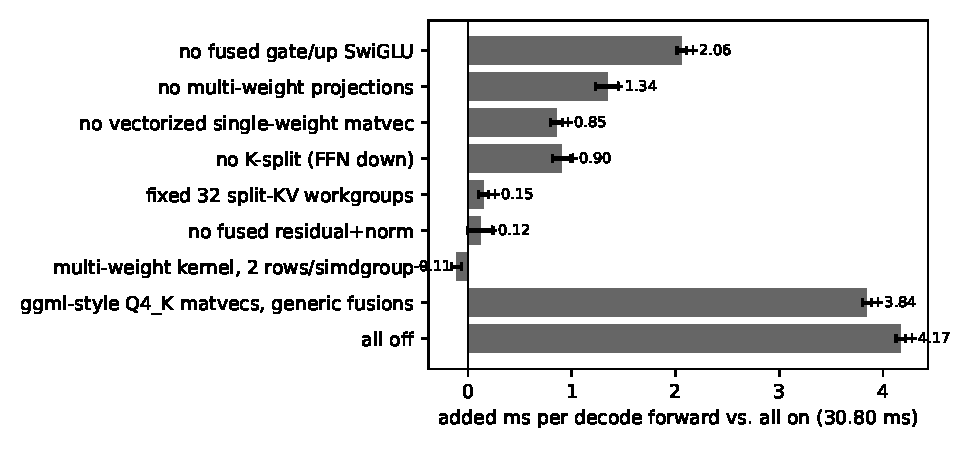
\includegraphics[width=0.8\linewidth]{figs/ablation.pdf}
\caption{Decode throughput with one optimization removed at a time.}
\label{fig:ablation}
\end{figure}

The fused gate/up kernel is the largest single item, followed by the
multi-weight projections; the vectorized single-weight matvec and the K-split
overlap because both replace the ggml-style kernel on the FFN down projection.
The residual+norm fusion and the context-scaled attention are small at a
40-token context and the sum of the switches (6.0~\tps{}) exceeds the
end-to-end difference (3.9) because several remove the same dispatch overhead.

\subsection{Context length and MLX}
Figure~\ref{fig:context} and Table~\ref{tab:context} sweep the prompt from
1.4k to 33k tokens. Decode falls from 32.3 to 26.8~\tps{} for \ds{} and from
23.6 to 20.3 for llama.cpp. The DeltaNet layers cost the same at every length
(Table~\ref{tab:stages}); the decline is the sixteen attention layers reading
a K/V cache that grows by 64~KiB per position summed over those layers, plus
the split-KV reduce (0.97 to 3.38~ms per token from 40 to 8.6k tokens).
Prefill throughput is the same in \ds{} and llama.cpp within 3\% at every
length: prefill is a matrix--matrix workload on comparable dequantize-and-multiply
kernels, and the model-specific graph does not pay there.

MLX is the informative comparison. Its 4-bit affine format (a 16-bit scale and
bias per group of 64, 4.5 bits per weight, the same as Q4\_K) decodes at
33.5~\tps{} at 1.4k context and stays within 2.3~\tps{} of \ds{} at every
length, from a general framework whose model code is a few hundred lines of
Python over its primitives; its prefill is 13--19\% slower. We read the decode
parity as a statement about the format, not the graph: affine dequantization
is a multiply-add per weight, and \S\ref{sec:anatomy} showed that the Q4\_K
matvecs are held below the Q8\_0 streaming rate by dequantization work.
\S\ref{sec:q40} tests this directly.

\begin{table}[t]
\centering
\begin{tabular}{rrrrrrr}
\toprule
 & \multicolumn{3}{c}{decode} & \multicolumn{3}{c}{prefill} \\
Prompt tokens & \ds{} & MLX & llama.cpp & \ds{} & MLX & llama.cpp \\
\midrule
1450 & 32.3 & 33.5 & 23.6 & 268 & 217 & 266 \\
4306 & 29.9 & 32.2 & 22.6 & 272 & 224 & 266 \\
8590 & 31.3 & 31.0 & 22.8 & 268 & 224 & 261 \\
17158 & 29.5 & 29.9 & 21.9 & 258 & 219 & 250 \\
32866 & 26.8 & 27.5 & 20.3 & 239 & 208 & 232 \\
\bottomrule
\end{tabular}
\caption{Throughput (\tps{}) versus prompt length, greedy, 64 decoded tokens,
single runs. \ds{} and llama.cpp on pure Q4\_K, MLX on its 4-bit affine
conversion. The 4k/8k inversion for \ds{} is within the $\pm1$~\tps{}
single-run spread at these lengths.}
\label{tab:context}
\end{table}

\begin{figure}[t]
\centering
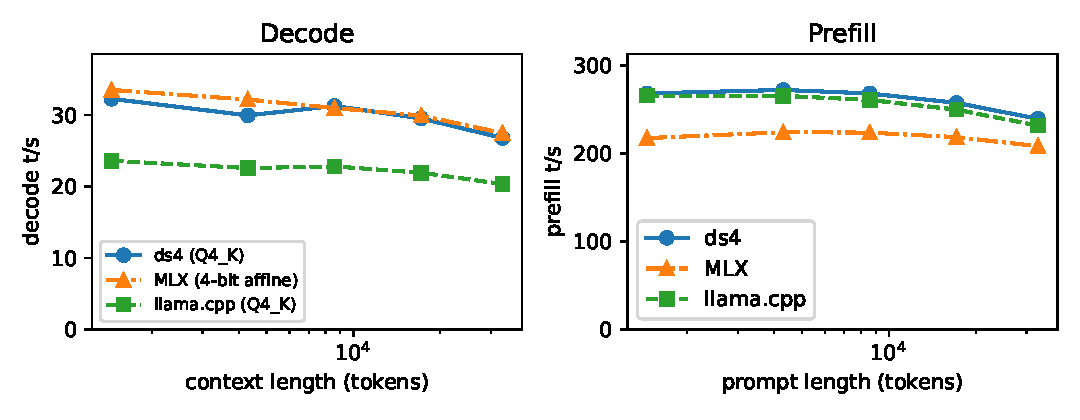
\includegraphics[width=\linewidth]{figs/context.pdf}
\caption{Decode and prefill throughput versus prompt length.}
\label{fig:context}
\end{figure}

\subsection{The format lever: Q4\_0 against Q4\_K}
\label{sec:q40}
To separate the quantization format from everything else we built a pure
Q4\_0 file from the same Q8\_0 source with the same importance matrix and the
same Q8\_0 output head as the pure Q4\_K file: identical bit budget (16.0~GB
on disk), different block layout. Q4\_0 stores one 16-bit scale per 32
weights and dequantizes with one multiply-add per weight; Q4\_K packs 6-bit
sub-block scales and minimums into a 256-weight super-block that must be
unpacked. We ported the ggml-style Q4\_0 matvec into \ds{} and then the fused
gate/up and multi-weight kernels; Table~\ref{tab:q40} gives the result at
each kernel level in both engines.

\begin{table}[t]
\centering
\begin{tabular}{llrr}
\toprule
Engine & Kernels & Q4\_K & Q4\_0 \\
\midrule
llama.cpp & stock & 23.8 & 28.4 \\
\ds{} & per-format ggml-style matvecs, generic fusions & 29.5 & 31.7 \\
\ds{} & + fused gate/up and multi-weight kernels & 33.1 & 33.6 \\
\midrule
wikitext-2 PPL & & $5.80 \pm 0.07$ & $6.03 \pm 0.07$ \\
\bottomrule
\end{tabular}
\caption{Decode \tps{} for the same weights in Q4\_K and Q4\_0 (both pure,
same imatrix, Q8\_0 head), greedy, 22-token prompt. ``Generic fusions'' are
the residual+norm fusion, the single prologue and the context-scaled
attention, which do not depend on the format. Q4\_0 logits agree with
llama.cpp to a mean $|\Delta|$ of 0.0009 at decode step 4.}
\label{tab:q40}
\end{table}

With simple kernels the format alone is worth 19\% in llama.cpp and 7\% in
\ds{}: the Q4\_0 gate/up pair streams at 171~$\mu$s per layer against 196
for Q4\_K. With the fused kernels the two formats land at 33.6 and
33.1~\tps{}. The stage profile explains why the gains do not compose: the
fused gate/up kernel takes 166~$\mu$s in Q4\_0 and 164 in Q4\_K, both about
610~GB/s, so once the largest projection is fused the cheaper dequantization
has nothing left to buy there. Q4\_0 still gains on the narrower projections
(84 against 94~$\mu$s for the DeltaNet projections, 75 against 82 for
attention) and loses on the FFN down projection (103 against 95), which has a
K-split kernel only for Q4\_K. The format lever therefore matters in
proportion to how far the kernels are from the streaming ceiling, and MLX's
34.1~\tps{} on the affine format sits at that same ceiling.

\subsection{A second family: mixture of experts}
\ds{} was written for DeepSeek V4 Flash, a mixture-of-experts model, and its
decode there is shaped by a different lever: only the routed experts of a
token are read, so bytes per token depend on routing, and the engine gathers
expert weights from a combined buffer and fuses the router with the
selection. On the 86~GB mixed-recipe file (IQ2\_XXS routed experts, Q8\_0
attention projections, shared experts and head), \ds{} decodes at
30.3~\tps{} against 25.2 for llama.cpp on the same file (greedy, short prompt,
64 tokens). Table~\ref{tab:moe} is the same profiler on this model. The routed
experts, the query path and the attention output projection account for two
thirds of the token, and no single projection dominates the way the FFN does
in the dense model; the decomposition applies per family with a different
dominant term, and the specific kernels do not transfer.

\begin{table}[t]
\centering
\small
\begin{tabular}{lrr}
\toprule
Profiler stage (43 layers) & $\mu$s/layer & ms/token \\
\midrule
\texttt{routed\_moe} & 201 & 8.65 \\
\texttt{q\_path} & 164 & 7.06 \\
\texttt{attn\_inv\_rope} & 134 & 5.75 \\
\texttt{attn\_output} & 117 & 5.05 \\
\texttt{router} & 51 & 2.18 \\
\texttt{kv\_path} & 32 & 1.36 \\
\texttt{attn\_hc\_pre}, \texttt{ffn\_hc\_pre} (hyper-connection mixes) & 26 each & 2.27 \\
\texttt{shared\_down} & 23 & 1.00 \\
compressor and indexer updates (amortized) & & 0.51 \\
\midrule
total & & 33.8 \\
\bottomrule
\end{tabular}
\caption{Per-stage GPU time for DeepSeek V4 Flash decode on \ds{}, 40-token
context, using the engine's stage labels. A stage whose kernels are encoded in
a neighbour's command buffer is attributed to that neighbour, which is why
some labels report zero and are omitted.}
\label{tab:moe}
\end{table}

\section{What did not work}
\label{sec:negative}
\paragraph{K-split on wide matrices.} Splitting the reduction across the
simdgroups of a threadgroup multiplies the thread count for a fixed number of
output rows. It helped only the long-row FFN down projection and was neutral
or slightly worse on the 10240- and 12288-output projections; occupancy was
not their limiter, the activation re-read per row was, and rows per
simdgroup was the parameter that moved.
\paragraph{Output gate fused into the attention reduce.} A copy of the
split-KV reduce that multiplies by $\sigma(\text{gate})$ before its single
store was consistently 20~$\mu$s per layer slower than the shared reduce
followed by a trivial elementwise gate kernel, even with the gate arithmetic
removed. The copy specializes its loops on function constants where the shared
kernel takes them as runtime arguments; we did not confirm that this is the
cause, and dropped the fusion.
\paragraph{Convolution folded into the recurrence.} Each of the 1,536
recurrence threadgroups would recompute the causal convolution for its head's
256 $q$/$k$ channels, a 32-fold redundant read of the convolution state. The
estimated cache traffic exceeded the one dispatch it would save.

\section{Discussion}
\label{sec:discussion}
\paragraph{Model-specific against generic.} \ds{} implements each supported
architecture as a hand-written graph. The cost is that each new family is a
port; the benefit is that every fusion above is a local change with a
measured effect and the per-token dispatch list is known and short. A generic
graph runner can obtain the same fusions from a pass over its graph, and
llama.cpp and MLX both fuse some operators, but the two decode-specific
fusions that mattered most here, batching a layer's side projections into one
launch and scaling the split-KV work to the context, are decisions about the
model and the session rather than about the graph. The MLX result shows that a
cheaper format buys the same as our kernel work at this scale; both together
would be the next step, and the engine now has the Q4\_0 kernels for it.
\paragraph{What is left.} The remaining 20\% to the ceiling is split between
the latency-bound recurrence, the attention path, and per-dispatch ramp;
\S\ref{sec:q40} shows that dequantization is no longer one of the terms once
the large matvecs are fused. Beyond that the model ships a multi-token
prediction head, and speculative decoding with it would verify two tokens per
weight pass; we have not implemented it.

\section{Related work}
\paragraph{Local inference runtimes.} llama.cpp and ggml~\cite{llamacpp,ggml}
are the reference for consumer-hardware inference; their Q4\_K and Q4\_0
matvecs are the starting points of the kernels we compare against, and their
split-KV decode attention is the one we adapt. MLX~\cite{mlx} is Apple's array
framework; mlx-lm~\cite{mlxlm} implements the Gated DeltaNet families on it.
\paragraph{Roofline and phase analyses.} Memory-bound decode and the
prefill/decode split are the basis of FlashAttention and
Flash-Decoding~\cite{dao2022flashattention,dao2023flashdecoding} and of
disaggregated serving~\cite{patel2024splitwise,zhong2024distserve}. Those
analyses target discrete GPUs; the unified-memory setting puts the CPU on the
inter-token critical path and makes per-dispatch cost visible at 27B scale.
\paragraph{Hybrid linear-attention models.} Gated
DeltaNet~\cite{yang2025gateddeltanet} and the Qwen3-Next and Qwen3.5
families~\cite{qwen3next,qwen35} interleave linear-attention layers with a
minority of softmax-attention layers; the reference CUDA kernels~\cite{yang2024fla}
use chunked and recurrent forms that do not transfer to Metal.
\paragraph{Quantization formats.} Weight-only quantization
methods~\cite{frantar2023gptq,lin2024awq}, the k-quant block
formats~\cite{kquants}, importance-matrix calibration~\cite{imatrix} and
mixed-recipe files~\cite{unslothdynamic} trade bytes for dequantization work;
\S\ref{sec:q40} measures that trade on Apple GPUs.
\paragraph{Speculative and multi-token decoding.} Verifying several tokens per
weight pass~\cite{leviathan2023fast,chen2023accelerating,cai2024medusa,li2024eagle}
is the standard route past the streaming bound; the model used here ships a
multi-token prediction head~\cite{gloeckle2024mtp,deepseekv3}.

\section{Limitations}
All results are from one machine, an M2~Ultra with a 60-core GPU. The
achieved bandwidth fractions and the balance between levers will differ on
other generations; in particular the M5 family adds GPU matrix units that
change the prefill regime, and a device sweep is the obvious extension. The
decomposition is for one dense hybrid family; the MoE result is a throughput
and a profile, not an ablation. The per-stage profiler perturbs what it
measures by isolating stages, so we use it for rankings and deltas only.
The sampler finding depends on compiler flags and may not reproduce under
\texttt{-fno-finite-math-only}. The downstream check has ten items.

\section{Conclusion}
A decode token on Apple silicon is not simply bandwidth bound at the 27B
scale: matvec kernel shape, dispatch count and CPU work between tokens each
cost milliseconds, and each needs its own measurement. Taking GPU timestamps
per stage and timing the CPU gap turned each optimization into a targeted
change with a known payoff, the switches make the account auditable, and the
controlled format experiment shows where one lever stops and another starts.

\bibliographystyle{plain}
\bibliography{refs}

\appendix
\section{Reproduction}
\label{sec:repro}
The code is our fork of the \ds{} repository~\cite{ds4} at \branchurl{}.
Three branches build on each other: \texttt{general-decode-fixes} (sampler and
diagnostics), \texttt{qwen38-support} (the model and its decode paths) and
\texttt{paper-artifact} (this document and the scripts under
\texttt{paper/scripts/}). Everything below was run on macOS 26.1 with
Xcode's command-line tools; a llama.cpp checkout is needed for the baselines,
the reference logits and the quantization.

\subsection*{1. Build}
\begin{lstlisting}
git clone https://github.com/parasol-aser/ds4 && cd ds4 && git checkout paper-artifact
make                                   # ds4, ds4-server, ds4-agent, ds4-eval
git clone https://github.com/ggml-org/llama.cpp ~/github/llama.cpp
cd ~/github/llama.cpp && git checkout 6d9c82ea2
cmake -B build && cmake --build build -j
pip3 install -U mlx-lm                 # 0.31.3 or later for the qwen3_5 architecture
\end{lstlisting}

\subsection*{2. Models}
\begin{lstlisting}
./download_model.sh qwen38-q8          # Qwen3.8-27B-Q8_0.gguf
./download_model.sh qwen38-q4km        # Qwen3.8-27B-UD-Q4_K_M.gguf
./download_model.sh ds4f-q2            # DeepSeek V4 Flash mixed-recipe file
# importance matrix from the same Unsloth release, then the two pure files:
cd gguf
curl -LO https://huggingface.co/unsloth/Qwen3.8-27B-GGUF/resolve/main/imatrix_unsloth.gguf
L=~/github/llama.cpp/build/bin
$L/llama-quantize --allow-requantize --pure --imatrix imatrix_unsloth.gguf \
  --output-tensor-type q8_0 --token-embedding-type q4_k \
  Qwen3.8-27B-Q8_0.gguf Qwen3.8-27B-Q4_K.gguf Q4_K_S 8
$L/llama-quantize --allow-requantize --pure --imatrix imatrix_unsloth.gguf \
  --output-tensor-type q8_0 --token-embedding-type q4_0 \
  Qwen3.8-27B-Q8_0.gguf Qwen3.8-27B-Q4_0.gguf Q4_0 8
\end{lstlisting}
The DeepSeek file we measured is the earlier build of the \texttt{ds4f-q2}
recipe (same name without the \texttt{-0731} suffix).

\subsection*{3. Reference logits}
\begin{lstlisting}
cd paper/scripts && mkdir -p out
c++ -std=c++17 -O2 -I ~/github/llama.cpp/include -I ~/github/llama.cpp/ggml/include \
  logits_dump.cpp -L ~/github/llama.cpp/build/bin -lllama -lggml -lggml-base \
  -Wl,-rpath,$HOME/github/llama.cpp/build/bin -o out/logits_dump
# reference: prefill, greedy, dump the logits of step 4
out/logits_dump ../../gguf/Qwen3.8-27B-Q4_K.gguf "$PROMPT" 8 5 4 out/ref_s4.bin
# ds4: same prompt, dump the logits of its 4th forward
DS4_GLM_LOGIT_DUMP=out/ds4_s4.bin DS4_QWEN_LOGIT_DUMP_STEP=4 \
  ../../ds4 -m ../../gguf/Qwen3.8-27B-Q4_K.gguf -p "$PROMPT" -n 8 --temp 0 -c 4096
python3 cmp.py out/ds4_s4.bin out/ref_s4.bin      # mean/max |diff|, argmax
\end{lstlisting}
\texttt{\$PROMPT} is the ChatML prompt with an empty thinking block, as in
\texttt{run\_all.sh}.

\subsection*{4. Experiments}
\begin{lstlisting}
cd paper/scripts
curl -sL -o out/wikitext-2-raw-v1.zip \
  https://huggingface.co/datasets/ggml-org/ci/resolve/main/wikitext-2-raw-v1.zip
unzip -qo out/wikitext-2-raw-v1.zip -d out
python3 make_prompts.py                # out/prompt_{1k,4k,8k,16k,32k}.txt
./run_all.sh                           # ~30 min: sweeps, ablation, profiles, PPL, MoE
./run_q40.sh                           # ~15 min: pure Q4_0 experiment
./run_mlx.sh                           # download (15 GB) + ~20 min
./run_eval.sh                          # ~40 min: downstream check
python3 analyze.py                     # tables; python3 figures.py -> ../figs/
\end{lstlisting}
The GPU must be otherwise idle: \ds{} refuses to start while another \ds{}
process holds \texttt{/tmp/ds4.lock}, and timing is not meaningful with a
second model process on the GPU.

\subsection*{5. Switches and profilers}
\begin{lstlisting}
DS4_METAL_DECODE_STAGE_PROFILE=1 DS4_METAL_CB_TIMES=1  # per-stage GPU spans
DS4_TOKEN_TIMING=1                       # CLI: sample / emit / eval per token
DS4_GLM_LOGIT_DUMP=f DS4_QWEN_LOGIT_DUMP_STEP=k   # logits of the k-th forward
DS4_QWEN_DISABLE_FUSED_SWIGLU=1   # fused gate/up -> two matvecs + SwiGLU
DS4_QWEN_DISABLE_MULTI_PROJ=1     # multi-weight proj -> one launch each
DS4_QWEN_DISABLE_FAST_MV=1        # vectorized single-weight mv -> ggml-style
DS4_METAL_Q4K_KSPLIT_NSG=0        # K-split (FFN down) off
DS4_METAL_QWEN_FA_NWG=32          # fixed 32 split-KV workgroups
DS4_QWEN_DISABLE_FUSED_NORM=1     # residual+norm fusion off
DS4_METAL_Q4K_MULTI_NR0=2         # multi-weight kernel rows per simdgroup
\end{lstlisting}
Stage-profile logs are aggregated with \texttt{stage\_agg.py}. The Metal
System Trace captures of \S\ref{sec:anatomy} were recorded and exported
with:
\begin{lstlisting}
xcrun xctrace record --template 'Metal System Trace' --time-limit 120s \
  --output ds4.trace --launch -- ./ds4 -m gguf/Qwen3.8-27B-UD-Q4_K_M.gguf -p "$PROMPT" -n 32 --temp 0
xcrun xctrace export --input ds4.trace \
  --xpath '/trace-toc/run[@number="1"]/data/table[@schema="metal-gpu-intervals"]'
xcrun xctrace export --input ds4.trace \
  --xpath '/trace-toc/run[@number="1"]/data/table[@schema="metal-application-command-buffer-submissions"]'
\end{lstlisting}
GPU busy fraction and per-token GPU time come from the union of the GPU
intervals in the decode window; CPU encode time per token from the submission
table's encoder durations.

\end{document}
